\documentclass[11pt,twoside]{scrartcl}
%\documentclass[11pt,twoside]{article}

%opening
\newcommand{\lecid}{15-316}
\newcommand{\leccourse}{Software Foundations of Security and Privacy}
\newcommand{\lecdate}{} %e.g. {October 21, 2013}
\newcommand{\lecnum}{6}
\newcommand{\lectitle}{Automated Safety-Checking Strategies}
\newcommand{\lecturer}{Matt Fredrikson}
\newcommand{\lecurl}{https://15316-cmu.github.io/index}

\usepackage{varwidth}
\usepackage{lecnotes}
\usepackage[irlabel]{bugcatch}

\usepackage{tikz}
\usetikzlibrary{automata,shapes,positioning,matrix,shapes.callouts,decorations.text,patterns,trees}

% \usepackage[bracketinterpret,seqinfers,sidenotecalculus]{logic}
% \newcommand{\I}{\interpretation[const=I]}

% \newcommand{\bebecomes}{\mathrel{::=}}
% \newcommand{\alternative}{~|~}
% \newcommand{\asfml}{F}
% \newcommand{\bsfml}{G}
% \newcommand{\cusfml}{C}
% \def\leftrule{L}%
% \def\rightrule{R}%

\begin{document}

\newcommand{\atrace}{\sigma}%
%% the standard interpretation naming conventions
\newcommand{\stdI}{\dTLint[state=\omega]}%
\newcommand{\Ip}{\dTLint[trace=\atrace]}%
\newcommand{\ws}{\omega}\newcommand{\wt}{\nu}% 

\maketitle
\thispagestyle{empty}

%%%%%%%%%%%%%%%%%%%%%%%%%%%%%%%%%%%%%%%%%%%%%%

\section{Introduction \& Recap}

In the previous lecture we looked into proving that programs satisfy safety properties given as formulas in the first-order dynamic logic. In particular, we can write contract properties with precondition $\ausfml$ and postconditions $\busfml$ for a program $\asprg$ as:
\begin{equation}
\ausfml \limply \dbox{\asprg}{\busfml}
\end{equation}
If this formula is valid, then it means that in every state $\omega$, if $\omega\models\ausfml$ then after all terminating runs of $\asprg$ starting in $\omega$ the final state $\nu\models\busfml$. 

We then defined the semantics of dynamic logic formulas, so that we can actually prove the validity of such formulas. However, this is not always such an easy thing to do because there are an infinite number of initial states to reason about. To address this we derived a set of axioms that can be used in sequent calculus proofs to reason about the validity of DL formulas. 

\begin{center}
  \begin{calculus}
\cinferenceRule[assignb|$\dibox{:=}$]{assignment / substitution axiom}
{\linferenceRule[equiv]
  {p(\astrm)}
  {\axkey{\dbox{\pupdate{\umod{x}{\astrm}}}{p(x)}}}
}
{}%{$genDJ{x}$ free for $x$ in $\ausfml$}
\cinferenceRule[assertb|$\dibox{\text{assert}}$]{assert}
{\linferenceRule[equiv]
  {(\ivr \land \ausfml)}
  {\axkey{\dbox{\passert{\ivr}}{\ausfml}}}
}{}%
\cinferenceRule[ifb|$\dibox{\text{if}}$]{if-thenelse}
{\linferenceRule[equiv]
  {(\ivr\limply\dbox{\ausprg}{\ausfml}) \land (\lnot\ivr\limply\dbox{\busprg}{\ausfml})}
  {\axkey{\dbox{\pif{\ivr}{\ausprg}{\busprg}}{\ausfml}}}
}{}%
\cinferenceRule[composeb|$\dibox{{;}}$]{composition} %``One step at a time axiom''
{\linferenceRule[equiv]
  {\dbox{\ausprg}{\dbox{\busprg}{\ausfml}}}
  {\axkey{\dbox{\ausprg;\busprg}{\ausfml}}}
}{}%
\cinferenceRule[whileiterateb|$\dibox{\text{unwind}}$]{unfold while loop}
{\linferenceRule[equiv]
  {\dbox{\pifs{\ivr}{\plgroup\ausprg;\pwhile{\ivr}{\ausprg}\prgroup}}{\ausfml}}
  {\axkey{\dbox{\pwhile{\ivr}{\ausprg}}{\ausfml}}}
}{}%
\cinferenceRule[unfold|$\dibox{\text{unfold}}$]{unfold while loop}
{\linferenceRule[equiv]
  {(\ivr\limply\dbox{\ausprg}{\dbox{\pwhile{\ivr}{\ausprg}}{\ausfml}}) \land (\lnot\ivr\limply\ausfml)}
  {\axkey{\dbox{\pwhile{\ivr}{\ausprg}}{\ausfml}}}
}{}%
  \end{calculus}
\end{center}

Each of these axioms reduces reasoning about formulas involving the box modality to reasoning about a series of simpler formulas, sometimes not involving modalities at all. Moreover, the axioms can be ``implemented'' as a syntactic transformation on formulas, and so automated by tools. When a sequence of syntactic transformations results in formulas that don't contain any box modalities, then the original DL validity question becomes one of validity of arithmetic formulas. It again becomes possible to automate by invoking a decision procedure for first-order arithmetic, and many good ones exist.

This is all very good, but not entirely true in all cases. In particular the axioms \irref{whileiterateb} and \irref{unfold} for dealing with loops do not actually simplify matters at all. Applying either of these axioms results in an equivalent DL formula that reasons about the safety of the first iteration of the loop, and then a DL formula that is a carbon copy of the original for the remaining iterations.

The way to deal with this properly is to reason about loop invariants, introducing an axiom that requires us to prove the correctness of the invariant and that it implies the postcondition. But loop invariants cannot in general be derived automatically, and we are interested in techniques that can be automated and implemented in tools.

Another way to deal with this is to apply \irref{whileiterateb} or \irref{unfold} repeatedly for a while, and simply cut the proof off at a certain point. This is equivalent to unrolling the loop some bounded number of times, and assuming that it will terminate before hitting that bound. If we can prove safety for all iterations up to the bound, then we know that any safety violation must occur on longer executions. This is not an ideal solution because we know nothing about the program's behavior past the unwinding bound, but it will certainly give us more assurance than we would have gotten by running a few test cases.

\section{Bounded Model Checking}

The principle behind bounded model checking is straightforward. First, pick a bound $N$ on the execution depth of the program. This bound can refer to the total number of commands that are executed, or to the number of times loops are unrolled. We will adopt the latter convention, as it frees us from the potential awkwardness of splitting compound commands like conditionals and loops partway through their bodies.

Having fixed an upper bound on the execution depth, proceed to check the safety property $\ausfml \limply \dbox{\asprg}{\busfml}$ by repeatedly applying \irref{composeb}, \irref{assignb}, \irref{assertb}, and \irref{ifb}, as well as the axioms from the propositinal sequent calculus when necessary. Whenever the proof reaches a point at which no further progress can be made because all box modalities contain outermost $\pwhile{\ivr}{\asprg}$ commands, then apply \irref{unfold} and repeat the above process on the loop body $\asprg$. When \irref{unfold} has been applied to each loop $N$ times, then replace each occurrence of $\dbox{\pwhile{\ivr}{\asprg}}{\ausfml}$ with $\ausfml$. Then proceed to close out the proof by reducing any remaining obligations to arithmetic formulas and applying the rule \irref{qear}.

The best way to understand how this works is to see it in action. Let's start off simple, supposing that we wish to verify the following up to a bound of $N=1$:
\[
x \ne 0 \limply \dbox{z:=0; \pwhile{y>0}{\plgroup \pifs{y\%2=1}{\plgroup z:=z+x \prgroup} x:=2*x; y:=y/2\prgroup}}{z \ne 0}
\]
To keep things easier to read, we will let $\asprg$ denote the body of the while loop. We proceed as follows.
\begin{sequentdeduction}[array]
\linfer[implyr] {
  \linfer[composeb] {
    \linfer[assignbeqr] {
      \lsequent{x \ne 0,z=0}{\dbox{\pwhile{y>0}{\asprg}}{z \ne 0}}
    } {
      \lsequent{x \ne 0}{\dibox{z:=0}\dbox{\pwhile{y>0}{\asprg}}{z \ne 0}}
    }
  } {
    \lsequent{x \ne 0}{\dbox{z:=0; \pwhile{y>0}{\asprg}}{z \ne 0}}
  }
} {
  \lsequent{}{x \ne 0 \limply \dbox{z:=0; \pwhile{y>0}{\asprg}}{z \ne 0}}
}
\end{sequentdeduction}
We can proceed no further in the proof without applying \irref{unfold}. So we proceed to unfold the loop, and apply non-loop axioms afterwards until we get stuck again.
\begin{sequentdeduction}
\linfer[unfold] {
  \linfer[andr] {
    \linfer[implyr] {
      \lsequent{x\ne0,z=0,y>0} {\dibox{\asprg}\dbox{\pwhile{y>0}{\asprg}}{z\ne0}} 
    } {
      \lsequent{x\ne0,z=0} {y>0\limply\dibox{\asprg}\dbox{\pwhile{y>0}{\asprg}}{z\ne0}} 
    }
    &\ \ \linfer[implyr] {
      \lsequent{x\ne0,z=0,y\le0} {z\ne0}
    } {
      \lsequent{x\ne0,z=0} {y\le0 \limply z\ne0}
    }
  } {
    \lsequent{x\ne0,z=0} {(y>0\limply\dibox{\asprg}\dbox{\pwhile{y>0}{\asprg}}{z\ne0}) \land (y\le0 \limply z\ne0)}
  }
} {
  \lsequent{x \ne 0,z=0}{\dbox{\pwhile{y>0}{\asprg}}{z \ne 0}}
}
\end{sequentdeduction}
At this point we can't help but notice that the branch of our proof with $y\le0$ in the assumptions has no path forward. The formula:
\begin{equation}
\label{eq:vcbug}
x \ne 0 \land z = 0 \land y \le 0 \limply z \ne 0
\end{equation}
simply is not a valid formula of arithmetic. So, we've found a bug. What's more, examining the sequent that we are unable to prove:
\begin{equation}
\lsequent{x\ne0,z=0,y\le0}{z\ne0}
\end{equation}
we can extract more useful information about the bug. In particular the context provided by our assumptions tells us exactly what conditions of the initial state need to hold in order for the program to produce a trace that violates the safety property. So if we take any values of $x,y,z$ that satisfy the assumptions $x\ne0 \land z=0 \land y\le0$ then we are guaranteed to ``exercise'' the bug. Such a set of inputs and its corresponding trace is called a \emph{counterexample} to the safety property, and is a useful artifact of model checkers when debugging programs in practice.

\paragraph{Back to basic axioms.}
In hindsight, perhaps this is not so impressive because one of our assumptions is $z=0$. We probably should have seen this coming, because the program begins by initializing $z$ in this way, and will only update it when the loop body is executed. Perhaps there are more bugs to uncover if we continue with the other branch of the loop. In the following, let $\bsprg$ denote the program $x:=2*x;y:=y/2$.
\begin{sequentdeduction}[array]
\small
\linfer[composeb] {
  \linfer[ifb] {
    \textcircled{1}
    !\textcircled{2}
  } {
    \lsequent{x\ne0,z=0,y>0} {\dibox{\pifs{y\%2=1}{\plgroup z:=z+x \prgroup}}\dibox{\bsprg}\dbox{\pwhile{y>0}{\asprg}}{z\ne0}} 
  }
} {
  \lsequent{x\ne0,z=0,y>0} {\dibox{\pifs{y\%2=1}{\plgroup z:=z+x \prgroup};\bsprg}\dbox{\pwhile{y>0}{\asprg}}{z\ne0}} 
}
\end{sequentdeduction}
The branch of the proof marked $\textcircled{1}$ continues below.
\begin{sequentdeduction}
\linfer[implyr] {
  \linfer[composeb] {
    \linfer[assignbeqr] {
      \linfer[assignbeqr] {
        \linfer[assignbeqr] {
          \lsequent{x\ne0,z=0,y>0,y\%2=1,z_1=z+x,x_1=2*x,y_1=y/2} {\dbox{\pwhile{y_1>0}{\asprg}}{z_1\ne0}}
        } {
          \lsequent{x\ne0,z=0,y>0,y\%2=1,z_1=z+x,x_1=2*x} {\dibox{y:=y/2}\dbox{\pwhile{y>0}{\asprg}}{z_1\ne0}}
        }
      } {
        \lsequent{x\ne0,z=0,y>0,y\%2=1,z_1=z+x} {\dibox{x:=2*x}\dibox{y:=y/2}\dbox{\pwhile{y>0}{\asprg}}{z_1\ne0}}
      }
    } {
      \lsequent{x\ne0,z=0,y>0,y\%2=1} {\dibox{z:=z+x}\dibox{x:=2*x}\dibox{y:=y/2}\dbox{\pwhile{y>0}{\asprg}}{z\ne0}}
    }
  } {
    \lsequent{x\ne0,z=0,y>0,y\%2=1} {\dibox{z:=z+x}\dibox{\bsprg}\dbox{\pwhile{y>0}{\asprg}}{z\ne0}}
  }
} {
  \lsequent{x\ne0,z=0,y>0} {y\%2=1 \limply \dibox{z:=z+x}\dibox{\bsprg}\dbox{\pwhile{y>0}{\asprg}}{z\ne0}}
}
\end{sequentdeduction}
And the branch of the proof marked $\textcircled{2}$ continues here.
\begin{sequentdeduction}
\linfer[implyr] {
  \linfer[composeb] {
    \linfer[assignbeqr] {
      \linfer[assignbeqr] {
        \lsequent{x\ne0,z=0,y>0,y\%2\ne1,x_1=2*x,y_1=y/2} {\dbox{\pwhile{y_1>0}{\asprg}}{z\ne0}}
      } {
        \lsequent{x\ne0,z=0,y>0,y\%2\ne1,x_1=2*x} {\dibox{y:=y/2}\dbox{\pwhile{y>0}{\asprg}}{z\ne0}}
      }
    } {
      \lsequent{x\ne0,z=0,y>0,y\%2\ne1} {\dibox{x:=2*x}\dibox{y:=y/2}\dbox{\pwhile{y>0}{\asprg}}{z\ne0}}
    }
  } {
    \lsequent{x\ne0,z=0,y>0,y\%2\ne1} {\dibox{x:=2*x;y:=y/2}\dbox{\pwhile{y>0}{\asprg}}{z\ne0}}
  }
} {
  \lsequent{x\ne0,z=0,y>0} {y\%2\ne1 \limply \dibox{x:=2*x;y:=y/2}\dbox{\pwhile{y>0}{\asprg}}{z\ne0}}
}
\end{sequentdeduction}
Now in both branches of the proof, we can't go any further without applying \irref{unfold}. We initially set our bound to $N=1$, and we've unrolled the loop exactly one time. 

\paragraph{Verification conditions.} So we proceed to replace the formula $\dbox{\pwhile{y>0}{\asprg}}{z\ne0}$ with $z\ne0$ on both branches, yielding the sequents:
\begin{align}
\label{eq:vseq1}
\lsequent{x\ne0,z=0,y>0,y\%2=1,z_1=z+x,x_1=2*x,y_1=y/2} {z_1\ne0} \\
\label{eq:vseq2}
\lsequent{x\ne0,z=0,y>0,y\%2\ne1,x_1=2*x,y_1=y/2}{z\ne0} 
\end{align}
The sequents shown in \ref{eq:vseq1} and \ref{eq:vseq2} are our remaining proof obligations: if they are valid, then we can conclude that the safety property holds on the program traces corresponding to the paths that generated these obligations.
\begin{itemize}
\item In the case of \ref{eq:vseq1}, the corresponding path enters the while loop (reflected by the assumption $y>0$ in the sequent), enters the body of the conditional (reflected by the assumption $y\%2=1$), and executes the remainder of the loop body stopping just before iterating again. 
\item In the case of \ref{eq:vseq2}, the corresponding path enters the while loop ($y>0$ is still in the assumptions), skips over the body of the conditional (reflected by $y\%2\ne1$), and executes the rest of the loop body stopping prior to another iteration.
\end{itemize}

Observe that in both cases the proof obligations involve nothing but arithmetic. Recalling the meaning of sequents, we can derive arithmetic formulas whose validity implies the correctness of these paths.
\begin{align}
\label{eq:vc1}
x\ne0 \land z=0 \land y>0 \land y\%2=1 \land z_1=z+x \land x_1=2*x \land y_1=y/2 &\limply z_1\ne0 \\
\label{eq:vc2}
x\ne0 \land z=0 \land y>0 \land y\%2\ne1 \land x_1=2*x \land y_1=y/2 &\limply z\ne0
\end{align}
Equations \ref{eq:vc1} and \ref{eq:vc2} are called \emph{verification conditions}. Recall from earlier Equation~\ref{eq:vcbug}, the formula whose invalidity told us that the program contains a bug whenever $x\ne0 \land z=0 \land y\le0$. This was also a verification condition, corresponding to the program path where the body of the while loop is skipped over immediately leading to termination.

The primary job of a bounded model checker is to generate verification conditions for each program path within the execution depth bound. This can be done fully automatically, because there is nothing particularly difficult about applying the axioms \irref{composeb}, \irref{assignbeqr}, \irref{assertb}, and \irref{ifb}. As each verification condition is derived, the bounded model checker consults an automated decision procedure for arithmetic. This often involves exploiting the duality between satisfiability and validity covered in the second lecture, as most decision procedures are designed to answer satisfiability queries rather than validity. But this is not a practical hurdle, as it merely involves negating the verification condition.

\paragraph{Other first-order theories.} So far in this course we have assumed that our programs operate over ``real'' unbounded integers. This means that the verification conditions that we generate are formulas in the first-order theory of integer arithmetic. This theory is defined by the interpretation given to the constants (0,1,2,\ldots), functions ($+,-,\times,\ldots$), and predicates ($\le,=,\ldots$). We expect that claims of validity for these formulas assume the usual interpretation for such entities that we are familiar with from arithmetic over the integers.

Programs written in languages like C do not operate over such integers. Rather, they operate over machine integers that have bounded with (i.e., 32 or 64 bits), and thus can only take values from a finite set that can be represented as binary numbers of the according width. Likewise, functions like addition and subtraction have a different interpretation over the machine integers, which for example manifest when the result of an operation is too large or too small to be represented by the width of the architecture (i.e., overflow and underflow). Machine integers have additional functions such as bitwise \verb'&' and \verb'|', and shift operators \verb'>>' and \verb'<<'.

Just as one can define a first-order theory of ``real'' integers, it is possible to define a first-order theory of machine integers, or perhaps floating-point decimal numbers, by assigning the appropriate interpretations to the constants, functions, and predicates pertinent to machine integers. Decision procedure developers of course realize this, and have indeed built support for such theories in widely-used tools. Bounded model checkers exploit this to faithfully model the semantics of machine arithmetic for languages like C by generating verification conditions for the first-order theory of machine integers. Importantly, \emph{doing so does not generally entail changes to the verification condition generator itself}, as this is a purely syntactic analysis that does not depend on the interpretation of the underlying term constructors!

Let's look at a quick example involving machine integer arithmetic to get a sense of the differences that might arise when reasoning about correctness and safety. Consider the following program, which diligently checks that the denominator is non-zero before using it.
\begin{lstlisting}[basicstyle=\small,style=customjava,escapechar=\#]
if(a>0 #$\lor$# b>0) {
  assert(a+b #$\ne$# 0);
  x := c/(a+b);
}
\end{lstlisting}
We can check that the safety property corresponding to the assertion holds by reasoning about the validity of $\dbox{\pifs{a>0 \lor b>0)}{\plgroup\passert{a+b\ne0};x:=c/(a+b)\prgroup}}{\mtrue}$, as follows.
\begin{sequentdeduction}
\linfer[ifb] {
  \linfer[composeb] {
    \linfer[assignb] {
      \linfer[assertb] {
        \lsequent{}{a>0 \lor b>0 \limply a+b\ne0}
      } {
        \lsequent{}{a>0 \lor b>0 \limply \dibox{\passert{a+b\ne0}} {\mtrue}}
      }
    } {
      \lsequent{}{a>0 \lor b>0 \limply \dbox{\passert{a+b\ne0}} \dibox{x:=c/(a+b)} {\mtrue}}
    }
  } {
    \lsequent{}{a>0 \lor b>0 \limply \dibox{\passert{a+b\ne0};x:=c/(a+b)}{\mtrue}}
  }
} {
  \lsequent{}{\dbox{\pifs{a>0 \lor b>0)}{\plgroup\passert{a+b\ne0};x:=c/(a+b)\prgroup}}{\mtrue}}
}
\end{sequentdeduction}
The last step follows because $a+b\ne0 \land \mtrue$ is equivalent to $a+b\ne0$. Now in the theory of integer arithmetic \irref{qear}, our verification condition
\begin{equation}
\label{eq:machinevc}
a>0 \lor b>0 \limply a+b\ne0
\end{equation}
is perfectly valid, and we could close out the proof by simply applying the rule \irref{qear}. But in the theory of 32-bit machine integer arithmetic, if $a$ and $b$ are unsigned then Eq.~\ref{eq:machinevc} is not valid. Consider the counterexample $a = 2^{32}-1 = \texttt{0xFFFFFFFF} = 4294967295$ and $b=1$. Then $a+b=0$ because the result $4294967296 = 2^{32}$ is too large to fit in a 32-bit unsigned integer representation, so the result of the addition wraps around to zero.

From now on, when we want to use the theory of machine integer arithmetic in our proofs, we will use the rule \irref{qmear}.

\paragraph{Unwinding assertions.} From what we've seen so far, bounded model checking gives us a certain limited kind of assurance about the safety of a program. Let's break it down into cases.
\begin{enumerate}
\item If the bounded model checker finds a bug, it can report a counterexample. If the verification condition generator was implemented correctly and the correct theory was used by the decision procedure to discharge the proof obligation leading to the bug, then we can be sure that there is actually a bug in our program. 

How do we know this? Recall the axioms used to generate the verification condition: \irref{composeb}, \irref{assignbeqr}, \irref{assertb}, \irref{ifb}, and \irref{unfold}. Each of these is an equivalence reducing one formula to another, so that if the resulting verification condition is valid, then the original formula is as well. Likewise, if the VC is \emph{not} valid, then the original formula was not either. If this isn't convincing enough, then most decision procedures will produce a counterexample to the VC, that we can construct an input to the program with and actually run to observe the bug.

\item If the bounded model checker does \emph{not} find a bug, then all that we can say with confidence is that there are no bugs on paths up to the execution depth bound. At least we can say this, again due to the fact that we have proved the axioms of dynamic logic to be valid equivalences. But importantly, we can't say that there are \emph{no} safety bugs in the program when the model checker fails to find one, as there could be a bug on some path past the depth bound. Likewise, it could just as well be the case that there are indeed no such bugs on longer paths, but we shouldn't take this view without solid evidence to back it up.
\end{enumerate}
The second case is unfortunate. If the model checker finds no bugs then we will probably want to follow up to see if we can convince ourselves that there are no safety violations, but how?

One simple approach that sometimes works in practice is to use an \emph{unwinding assertion}. As the name suggests, an unwinding assertion is an assertion command that is added to the program as the bounded model checker applies the \irref{unfold} axiom. Whenever the depth bound is reached, rather than replacing $\dbox{\pwhile{\ivr}{\asprg}}{\ausfml}$ with $\ausfml$, $\dbox{\pwhile{\ivr}{\asprg}}{\ausfml}$ is replaced with $\dbox{\passert{\lnot\ivr}}{\ausfml}$. This way, verification will only succeed if the program would have terminated anyway after the bound was reached because $\lnot\ivr$ is true at that point. Let's look at a short example to illustrate the idea. We will set a depth bound of $N=2$ in the following proof.
\begin{sequentdeduction}
\linfer[unfold] {
  \linfer[andr] {
    \linfer[implyr] {
      \linfer[assignbeqr] {
        \linfer {
          \vdots
        } {
          \lsequent{x=2,0<x,x_1=x-1}{\dbox{\pwhile{0<x_1}{x_1:=x_1-1}}{x_1=0}}
        }
      } {
        \lsequent{x=2,0<x}{\dibox{x:=x-1}\dbox{\pwhile{0<x}{x:=x-1}}{x=0}}
      }
    } {
      \lsequent{x=2}{0 \le x \limply \dibox{x:=x-1}\dbox{\pwhile{0<x}{x:=x-1}}{x=0}}
    }
    &\ \ \linfer[qmear]{\lclose}{\lsequent{x=2}{0\ge x \limply x=0}}
  } {
    \lsequent{x=2}{(0 \le x \limply x:=x-1;\dbox{\pwhile{0<x}{x:=x-1}}{x=0}) \land (0\ge x \limply x=0)}
  }
} {
  \lsequent{x=2}{\dbox{\pwhile{0<x}{x:=x-1}}{x=0}}
}
\end{sequentdeduction}
We continue with the proof below, as we have run out of space. Let $P$ denote our assumptions so far $x=2,0<x,x_1=x-1$. This time when we apply \irref{unfold}, we will hit the execution bound immediately, and at that point insert the unwinding assertion.
\begin{sequentdeduction}
\linfer[unfold] {
  \linfer[andr] {
    \linfer[implyr] {
      \linfer[assignbeqr] {
        \linfer[assertb] {
          \lsequent{P,0<x_1,x_2=x_1-1}{0\ge x_2 \land x_2=0}
        } {
          \lsequent{P,0<x_1,x_2=x_1-1}{\dbox{\passert{0\ge x_2}}{x_2=0}}
        }
      } {
        \lsequent{P,0< x_1}{\dibox{x_1:=x_1-1}\dbox{\passert{0\ge x_1}}{x_1=0}}
      }
    } {
      \lsequent{P}{0<x_1 \limply \dibox{x_1:=x_1-1}\dbox{\passert{0\ge x_1}}{x_1=0}} 
    }
    &\ \ \linfer[qmear] {
      \lclose
    } {
      \lsequent{P}{0\ge x_1 \limply x_1 = 0}
    }
  } {
    \lsequent{P}{(0<x \limply \dibox{x_1:=x_1-1}\dbox{\passert{0\ge x_1}}{x_1=0}) \land (0\ge x_1 \limply x_1 = 0)}
  }
} {
  \lsequent{P}{\dbox{\pwhile{0<x_1}{x_1:=x_1-1}}{x_1=0}}
}
\end{sequentdeduction}
Now we have reduced the problem to machine arithmetic, leading to the verification condition
\begin{equation}
x=2 \land 0<x \land x_1 = x-1 \land 0<x_1 \land x_2=x_1-1 \limply 0\ge x_2 \land x_2=0
\end{equation}
This is of course valid, and because of the unwinding condition we know that there are no paths in the program that exceed the execution depth $N=2$. From this we conclude that the program satisfies the safety property on \emph{all} traces.

\section{Symbolic Execution}

Recall that when we discussed verification conditions, we saw that the assumptions in the context of each proof obligation reflect the path covered by that proof obligation. Also worth noting is that because we used \irref{assignbeqr} rather than \irref{assignb}, moving assignments to the assumptions and renaming variables each time, the context also tracks the intermediate state rather explicitly. Consider for example the following derivations.
\begin{sequentdeduction}[array]
\linfer[composeb+composeb] {
  \linfer[assignb] {
    \linfer[assignb] {
      \linfer[assignb] {
        \lsequent{x=a,y=b} {y=b\land x=a}
      } {
        \lsequent{x=a,y=b} {\dibox{z:=x}{y=b\land z=a}}
      }
    } {
      \lsequent{x=a,y=b} {\dibox{z:=x}\dibox{x:=y}{x=b\land z=a}}
    }
  } {
    \lsequent{x=a,y=b} {\dibox{z:=x}\dibox{x:=y}\dibox{y:=z}{x=b\land y=a}}
  }
} {
  \lsequent{x=a,y=b} {\dbox{z:=x; x:=y; y:=z}{x=b\land y=a}}
}
\end{sequentdeduction}
In this case, the verification condition is simply 
\begin{equation}
\label{eq:symbvc1}
x=a\land y=b \limply y=b \land x=a
\end{equation} 
All of the information about the intermediate states that the program entered to achieve its final result is gone from the condition. On the other hand, using \irref{assignbeqr} to do a similar derivation:
\begin{sequentdeduction}
\linfer[composeb+composeb] {
  \linfer[assignbeqr] {
    \linfer[assignbeqr] {
      \linfer[assignbeqr] {
        \lsequent{x=a,y=b,z_1=x,x_1=y,y_1=z_1} {x_1=b\land y_1=a}
      } {
        \lsequent{x=a,y=b,z_1=x,x_1=y} {\dibox{y:=z_1}{x_1=b\land y=a}}
      }
    } {
      \lsequent{x=a,y=b,z_1=x} {\dibox{x:=y}\dibox{y:=z_1}{x=b\land y=a}}
    }
  } {
    \lsequent{x=a,y=b} {\dibox{z:=x}\dibox{x:=y}\dibox{y:=z}{x=b\land y=a}}
  }
} {
  \lsequent{x=a,y=b} {\dbox{z:=x; x:=y; y:=z}{x=b\land y=a}}
}
\end{sequentdeduction}
Now the verification condition is
\begin{equation}
\label{eq:symbvc2}
x=a \land y=b \land z_1=x \land x_1 = y \land y_1=z_1 \limply x_1=b \land y_1=a
\end{equation}
In terms of reasoning about correctness, there is no difference here. Equations~\ref{eq:symbvc1} and \ref{eq:symbvc2} are equivalent. But the context tells us that the most recent ``version'' of $y$ (i.e. $y_1$) was updated to take the most recent version of $z$ (i.e. $z_1$), which was in turn updated to take the initial version of $x$.

\paragraph{Path formulas.}
The conjunction of the assumptions calculated in this way is called the \emph{path formula} for the corresponding program path behind this derivation. Any feasible path through a program has a corresponding path formula that is satisfiable. \emph{Symbolic execution} is a technique that enumerats program paths that may contain safety violations, generates their path formulas, and checks each formula for satisfiability. Whenever a path formula is satisfiable, it means that there is at least one trace that follows that path. 

To facilitate enumerating path formulas, symbolic execution first constructs a \emph{control flow graph} of the program that reflects all of the paths in the program. Consider the following program as an example.
\begin{lstlisting}[basicstyle=\small,style=customjava,escapechar=\#]
if(a > 0) { x := -2; }
if(b < 5) {
  if(a #$=$# 0 #$\land$# c #$\ne$# 0) { y:= 1 }
  z := 2;
}
assert(x+y+z #$\ne$# 3);
\end{lstlisting}
The corresponding control flow graph is as follows.
\begin{center}
\scalebox{1.1}{%
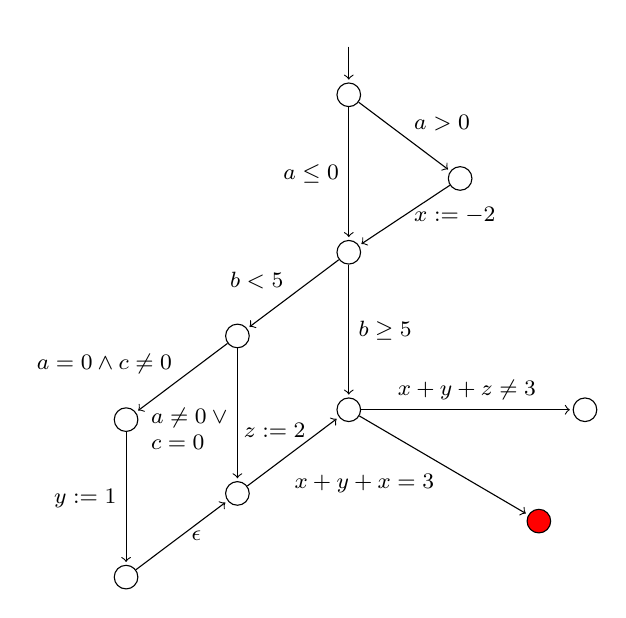
\begin{tikzpicture}
[
  highlight/.style={draw=blue, text=blue},
  shorten >=1pt,
  node distance=2cm,
  on grid,
  auto,
  /tikz/initial text={},
  font=\footnotesize
]
 \node[state,initial above,inner sep=1pt,minimum size=0.3cm] (l0)  {};
 \node[state,inner sep=1pt,minimum size=0.3cm,yshift=1em] (l1) [below right=of l0] {};
 \node[state,inner sep=1pt,minimum size=0.3cm] (l2) [below=of l0] {};
 \node[state,inner sep=1pt,minimum size=0.3cm,yshift=1em] (l3) [below left=of l2] {};
 \node[state,inner sep=1pt,minimum size=0.3cm] (l4) [below=of l2] {};
 \node[state,inner sep=1pt,minimum size=0.3cm,yshift=1em] (l5) [below left=of l3] {};
 \node[state,inner sep=1pt,minimum size=0.3cm] (l6) [below=of l5] {};
 \node[state,inner sep=1pt,minimum size=0.3cm] (l7) [below=of l3] {};
 \node[state,inner sep=1pt,minimum size=0.3cm,fill=red,xshift=1cm] (l8) [below right=of l4] {};
 \node[state,inner sep=1pt,minimum size=0.3cm,xshift=1cm] (l9) [right=of l4] {};

  \path[->] 
    (l0) edge node [left] {$\ptest{a\le 0}$} (l2)
    (l0) edge node [right,yshift=0.5em] {$\ptest{a>0}$} (l1)
    (l1) edge node [right] {$x:=-2$} (l2)
    (l2) edge node [left,yshift=0.5em] {$\ptest{b<5}$} (l3)
    (l2) edge node [right] {$\ptest{b\ge5}$} (l4)
    (l3) edge node [left,yshift=0.5em] {$\ptest{a=0\land c\ne0}$} (l5)
    (l5) edge node [left] {$y:=1$} (l6)
    (l6) edge node [right] {$\epsilon$} (l7)
    (l3) edge node [left,yshift=-0.5em] 
      {%
        \begin{varwidth}{1cm}
        $a\ne0\lor c=0$
        \end{varwidth}
      } (l7)
    (l7) edge node [left,yshift=0.75em,xshift=0.8em] {$z:=2$} (l4)
    (l4) edge node [above] {$\ptest{x+y+z\ne3}$} (l9)
    (l4) edge node [left,yshift=-0.65em] {$\ptest{x+y+x=3}$} (l8);
\end{tikzpicture}
}
\end{center}
The edges of the control flow graph are labeled to reflect the corresponding program command on that portion of the path. As shorthand, we write $\ptest{\ausfml}$ to represent conditions that must hold, i.e. in place of $\passert{\ausfml}$. The node marked in red denotes a path that violates the assertion. Edges labeled with $\epsilon$ are noops, and don't correspond to any program command. Then the task of symbolic execution is to determine if this node is reachable from an initial state from a feasible path.

Each path through the control flow graph corresponds to a verification condition, which we obtain by listing out a corresponding program for that path and then applying the relevant axioms of dynamic logic. For example, the path that first takes the right edge from the initial state, and then left edges until reaching the red node would be:
\begin{equation}
\lsequent{}{\dbox{\ptest{a>0};x:=-1;\ptest{b<5};\ptest{a=0\land c\ne0};y:=1;z:=2;\ptest{x+y+z=3}}{\mtrue}}
\end{equation}
Notice that we use the trivial postcondition $\mtrue$ because we are merely interested in whether there are \emph{any} traces that could follow this path. So we don't care what properties the final state may have, which is described by $\mtrue$. Applying axioms \irref{assignbeqr} and \irref{assertb}, we derive the following verification condition.
\begin{equation}
a>0 \land x_1 = -1 \land b < 5 \land a = 0 \land c\ne0 \land y_1 = 1 \land z_1 = 2 \land x_1 + y_1 + z_1 = 3
\end{equation}
This formula is not satisfiable, because $a>0 \land a=0$ is a contradiction, so there are no feasible traces that follow this path. On the other hand, if we had taken the left branch off of the initial state and then followed the same commands afterwards, it is not hard to check that we would obtain the following verification condition.
\begin{equation}
\label{eq:goodvc}
a\le 0 \land b < 5 \land a = 0 \land c\ne0 \land y_1 = 1 \land z_1 = 2 \land x + y_1 + z_1 = 3
\end{equation}
Equation~\ref{eq:goodvc} is indeed satisfiable, as evidenced by the witness $x=0,y_1=1,z_1=2$. This means that the path is feasible, which we could show by running the program on any input with $x=0$.

\paragraph{Checking invariants.}
Path formulas contain all of the information that we need to reason about the satisfaction of formulas over state at all points in the execution. For example, suppose we wish to check the invariant $\ausfml$. Part way through the derivation of 
\[
\lsequent{x=a,y=b} {\dbox{z:=x; x:=y; y:=z}{x=b\land y=a}}
\]
we derived the sequent $\lsequent{x=a,y=b,z_1=x}{\dibox{x:=y}\dbox{y:=z}{x=b \land y=a}}$. The context $x=a,y=b,z_1=x$ reflects the state after the first assignment $z:=x$. We need to show that at this point in the execution, $P$ holds, i.e., we can prove validity of:
\[
\lsequent{x=a,y=b,z_1=x}{\ausfml}
\]
Executing the next assignment $x:=y$ lead to the context $x=a,y=b,z_1=x,x_1=y$ and the obligation to prove:
\[
\lsequent{x=a,y=b,z_1=x,x_1=y}{\ausfml}
\]
And finally, executing the last assignment $y:=z$ gives the obligation:
\[
\lsequent{x=a,y=b,z_1=x,x_1=y,y_1=z_1}{\ausfml}
\]
This is a useful tactic, and the ability to select paths from the program affords more flexibility than bounded model checking the program:
\[
z:=x;\passert{P};x:=y;\passert{P};y:=z;\passert{P}
\]
This flexibility is important when the program is too large to perform bounded model checking on to a sufficiently large execution depth. If we can reason efficiently that there is a subset of paths on which the safety property will definitely hold, then the remaining (hopefully much smaller or at least finite) set of paths can be enumerated with symbolic execution and discharged individually. In subsequent lectures, we will see how runtime safety checks can be used to ensure that certain paths will never violate safety, so that targeted techniques like symbolic execution can be used to reason about the rest.

\end{document}